\documentclass[a4paper,12pt]{book}
\usepackage{polski}
\usepackage[utf8]{inputenc}
\usepackage[T1]{fontenc}  
\usepackage[margin=1in,left=1.5in,includefoot]{geometry}
\usepackage{fancyhdr}
\usepackage{wrapfig}
\usepackage{amsmath,amsfonts,amssymb,amsthm}
\usepackage[british,polish]{babel} 
\usepackage{indentfirst}
\usepackage{lmodern}
\usepackage{graphicx} 
\usepackage{hyperref}
\usepackage{booktabs}
\usepackage{tikz}
\usepackage{pgfplots}
\usepackage{mathtools}
\usepackage{geometry}
\usepackage{listings}
\pagestyle{fancy}
\usepackage{graphicx}
\graphicspath{ {./images/} }
%%%%%%%%%%%% ZYWA PAGINA %%%%%%%%%%%%%%%
% brak kapitalizacji zywej paginy
\usepackage{fancyhdr}
\pagestyle{fancy}
\fancyhf{}
\fancyhead[LO]{\nouppercase{\it\rightmark}}
\fancyhead[RE]{\nouppercase{\it\leftmark}}
\fancyhead[LE,RO]{\it\thepage}


\fancypagestyle{tylkoNumeryStron}{%
   \fancyhf{} 
   \fancyhead[LE,RO]{\it\thepage}
}

\fancypagestyle{NumeryStronNazwyRozdzialow}{%
   \fancyhf{} 
   \fancyhead[LO]{\nouppercase{\it\rightmark}}
   \fancyhead[RE]{\nouppercase{\it\leftmark}}
   \fancyhead[LE,RO]{\it\thepage}
}
\newcounter{stronyPozaNumeracja}

\newcommand{\hcancel}[1]{%
    \tikz[baseline=(tocancel.base)]{
        \node[inner sep=0pt,outer sep=0pt] (tocancel) {#1};
        \draw[red] (tocancel.south west) -- (tocancel.north east);
    }%
}%


\lstdefinelanguage[ECMAScript2015]{JavaScript}[]{JavaScript}{
  morekeywords=[1]{await, async, case, catch, class, const, default, do,
    enum, export, extends, finally, from, implements, import, instanceof,
    let, static, super, switch, throw, try},
  morestring=[b]` % Interpolation strings.
}


%
% JavaScript version 1.1 by Gary Hammock
%
% Reference:
%   B. Eich and C. Rand Mckinney, "JavaScript Language Specification
%     (Preliminary Draft)", JavaScript 1.1.  1996-11-18.  [Online]
%     http://hepunx.rl.ac.uk/~adye/jsspec11/titlepg2.htm
%

\lstdefinelanguage{JavaScript}{
  morekeywords=[1]{break, continue, delete, else, for, function, if, in,
    new, return, this, typeof, var, void, while, with,  public, private, protected, constructor, abstract },
  % Literals, primitive types, and reference types.
  morekeywords=[2]{false, null, true, boolean, number, string, undefined,
    Array, Boolean, Date, Math, Number, String, Object},
  % Built-ins.
  morekeywords=[3]{eval, parseInt, parseFloat, escape, unescape, length},
  sensitive,
  morecomment=[s]{/*}{*/},
  morecomment=[l]//,
  morecomment=[s]{/**}{*/}, % JavaDoc style comments
  morestring=[b]',
  morestring=[b]"
}[keywords, comments, strings]


\lstalias[]{ES6}[ECMAScript2015]{JavaScript}

% Requires package: color.
\definecolor{mediumgray}{rgb}{0.3, 0.4, 0.4}
\definecolor{mediumblue}{rgb}{0.0, 0.0, 0.8}
\definecolor{forestgreen}{rgb}{0.13, 0.55, 0.13}
\definecolor{darkviolet}{rgb}{0.58, 0.0, 0.83}
\definecolor{royalblue}{rgb}{0.25, 0.41, 0.88}
\definecolor{crimson}{rgb}{0.86, 0.8, 0.24}

\lstdefinestyle{JSES6Base}{
  backgroundcolor=\color{white},
  basicstyle=\ttfamily,
  breakatwhitespace=false,
  breaklines=false,
  captionpos=b,
  columns=fullflexible,
  commentstyle=\color{mediumgray}\upshape,
  emph={},
  emphstyle=\color{crimson},
  extendedchars=true,  % requires inputenc
  fontadjust=true,
  frame=single,
  identifierstyle=\color{black},
  keepspaces=true,
  keywordstyle=\color{mediumblue},
  keywordstyle={[2]\color{darkviolet}},
  keywordstyle={[3]\color{royalblue}},
  numbers=left,
  numbersep=5pt,
  numberstyle=\tiny\color{black},
  rulecolor=\color{black},
  showlines=true,
  showspaces=false,
  showstringspaces=false,
  showtabs=false,
  stringstyle=\color{forestgreen},
  tabsize=2,
  title=\lstname,
  upquote=true  % requires textcomp
}

\lstdefinestyle{JavaScript}{
  language=JavaScript,
  style=JSES6Base
}
\lstdefinestyle{ES6}{
  language=ES6,
  style=JSES6Base
}

\begin{document}

\begin{titlepage}

\title{Praca inżynierska}
\author{Kamil Susek}
\date{September 2020}

\maketitle
\end{titlepage}
\chapter{Wstęp}

Rozwój technologii pozwala na tworzenie coraz większych i bezpieczniejszych systemów, co prowadzi do przenoszenia niektórych procesów do świata wirtualnego. Takie działania pozwalają na zwiększenie efektywności i zmniejszenie kosztów tych procesów. Dodatkowo wyeliminowanie wpływu czynnika ludzkiego zwiększa wiarygodność takiego procesu i poprawia bezpieczeństwo. Przykładem takiego procesu jest głosowanie, które w tradycyjnej formie jest czasochłonne i trudne w organizacji. Natomiast przykładem technologii, która doprowadziła do prawdziwej rewolucji jest Blockchain. Blockchain odpowiada za przełomowe rozwiązanie w sektorze finansów, jakim jest Bitcoin, który zapoczątkował rozwój dużych systemów odpowiedzialnych za istotne procesy życia społecznego.

Tematem niniejszej pracy jest E-voting, czyli system głosowania przez internet, który będzie wspierany przez technologię Blockchain. W ramach pracy został przedstawiony teoretyczny model systemu, którego część zaimplementowano. Do zaimplementowanej części systemu należą: aplikacje internetowe wyborcy i organizatora oraz grupa serwisów dostarczających REST-owe API. Aplikacje wyborcy pozwala na zalogowanie się, wysłanie głosu i uzyskanie wyników wyborów. Natomiast aplikacja organizatora dostarcza narzędzia do konfiguracji i nadzorowania procesu wyborczego. Dostarczono również możliwość konfigurowania sieci Blockchain, która jest odpowiedzialna za zapisanie dodawanych głosów. Przez konfigurację sieci Blockchain rozumiane jest tworzenie sieci Peer-to-Peer.

W rozdziale pierwszym zostały przybliżone cele projektu i jego założenia, a także zakres pracy. Rozdział drugi poświęcony jest analizie dziedziny pracy, w tym rozdziale znajdują się informacje teoretyczne dotyczące technologii Blockchain, przykłady jej zastosowania oraz analiza istniejących rozwiązań E-votingu. Rozdział trzeci dotyczy opisu systemu od strony inżynierii oprogramowania. W tym rozdziale znajdują się informacje o wymaganiach projektu, przypadkach użycia oraz użytych narzędziach i technologiach. Rozdział czwarty dotyczy specyfikacji zewnętrznej systemu. Główne treści tego rozdziału to sposób korzystania z aplikacji, instrukcje dotyczące użytkowników systemu i sposób instalacji. Rozdział piąty dotyczy opisu architektury systemu, opisu algorytmów i szczegółów implementacji ciekawych fragmentów systemu. W szóstym rozdziale umieszczono wszystkie informacje dotyczące testowania oraz wykrytych błędów.
Ostatni rozdział, czyli rozdział siódmy poświęcony jest podsumowaniu całej pracy, w tym rozdziale znajdują się uzyskane wyniki i wnioski, a także możliwości dalszego rozwoju pracy.

\section{Cele i założenia pracy}

Celem pracy jest opracowanie oraz zaimplementowanie systemu, który umożliwia przeprowadzenie wyborów przez internet. Głównym założeniem projektu jest wykorzystanie technologii Blockchain. Zakres pracy obejmuje:

\begin{itemize}
	\item Analizę dziedziny i przegląd literatury dotyczącej wyborów internetowych i technologii Blockchain;
	\item Opracowanie systemu wyborów internetowych od strony teoretycznej;
	\item Implementację wybranej części całego systemu;
	\item Przetestowanie aplikacji.
\end{itemize}

\chapter{Wstępna analiza dziedziny}
Elektroniczne systemy głosowania coraz bardziej zyskują na popularności.
Wraz z postępem technologii oraz coraz większego znaczenia internetu w życiu 
społecznym, pojawiają się pomysły przeniesienia procesu głosowania do sieci. Pomysły i implementacje internetowych systemów wyborczych dotyczą wyborów na szczeblu państwowym (przykładowo wybory parlamentarne), jak i wyborów organizowanych na potrzeby prywatne. System e-votingu zazwyczaj sprowadza się do serwisu internetowego, który pozwala na oddanie głosu poprzez odpowiednią stronę internetową, bądź aplikację desktopową. 

Przeniesienie głosowania do aplikacji internetowej, pozwala zminimalizować wpływ ewentualnego błędu ludzkiego podczas przeprowadzania wyborów. Jednakże takie rozwiązanie generuje nowe problemy, z którymi muszą się zmierzyć projektanci tych systemów. Największy problem stanowi zabezpieczenie aplikacji, przed zewnętrznymi próbami fałszowania wyników głosowania. Rozwój technologii prowadzi również do powstawania nowych odmian “złośliwego oprogramowania”, co prowadzi do ciągłego aktualizowania zabezpieczeń. Aplikacja odpowiadająca na potrzeby wyborów, na wysokim szczeblu powinna być tworzona “na potrzeby danych czasów”, bądź łatwa w płynnej aktualizacji.

Zabezpieczenie przed fałszowaniem głosów to nie jest jedyny problem, z jakim trzeba się zmierzyć podczas próby przeniesienia procesu głosowania do internetu. Kolejnym problemem jest sama logika systemu głosowania, niektóre wybory wymagają, aby informacje o wyborcach oraz ich głosach, były tajne. System powinien również umożliwiać weryfikację użytkownika, na podstawie dostarczonych przez organizatora wyborów danych logowania. Coraz głębsza analiza problemu generuje coraz więcej potrzeb z zakresu bezpieczeństwa systemu. Dodatkowo wyszczególniając elementy, które powinny podlegać szczególnej protekcji należy zadbać, aby architektura systemu pozwalała na łatwą aktualizację zabezpieczeń.

Wykorzystując komputery do obsługi głosowania, oczekuje się szybkiego i poprawnego uzyskania rezultatu głosowania. System taki powinien być zoptymalizowany, a czas uzyskania rezultatów powinien być zdeterminowany. Warto rozważyć także moduł generujący statystyki wyborcze.

System wyborczy to nie tylko serwer, który zbiera, przechowuje i liczy głosy. Kliencka część aplikacji (widoczna dla wyborcy) powinna być responsywna, przejrzysta oraz przyjazna dla osób z pewnymi niepełnosprawnościami.

Dużą zaletą e-votingu jest przeniesienie procedur, które musi wykonać organizator do interaktywnej aplikacji przeglądarkowej. Aplikacja webowa powinna zapewniać możliwość zarządzania głosowaniem oraz kreator głosowania, ten element również powinien podlegać zabezpieczeniu danych i autentykacji użytkownika. Aplikacja wyposażona w takie funkcjonalności powinna spełniać wymagania elektronicznego systemu głosowania.

\section{Wstępne wymagania niefunkcjonalne}
Z powyższej analizy można wypunktować następujące wymagania:
\begin{itemize}

\item Dbałość o zabezpieczenie głosu wyborcy przed fałszerstwem - rezultat głosu nie może zostać zmieniony, po jego zatwierdzeniu.

\item Zabezpieczenie danych wyborcy, poprzez utajnienie jego tożsamości.

\item Sprawne i bezbłędne liczenie głosów - czas liczenia głosów powinien być deterministyczny.

\item Dbałość o stronę wizualną aplikacji, strona kliencka powinna być przejrzysta i łatwa w obsłudze.

\item System musi być konfigurowalny, z uwzględnieniem bezpieczeństwa konfiguracji.
\end{itemize}



\chapter{Blockchain}
Podstawy teoretyczne technologii Blockchain powstały już w roku 1991, a zostały opracowane przez dr Stuart'a Haber'a oraz dr W. Scott Stornetta. Naukowcy zajmowali się opracowaniem systemu, zabezpieczającego cyfrowe dokumenty przed podrobieniem, bądź podmianą. System opierał się na łańcuchach bloków, gdzie w każdym bloku znajdowały się cyfrowe dane dokumentu. Podczas dodawania nowego dokumentu do łańcucha, podpisywano go za pomocą tak zwanego stempla czasu (ang. timestamp), a następnie dokument był łączony z poprzednim dokumentem. Łączenie polega na przypisaniu nowem blokowi, wskaźnika na poprzedni dokument. Wartością wskaźnika były określone dane poprzedniego dokumentu, co stanowiło zabezpieczenie dokumentów. Jeżeli zawartość dokumentu w łańcuchu uległaby zmianie, to należałoby zmienić również wskaźnik na ten dokument\cite{pa}.

Kamieniem milowym w popularyzacji tego pomysłu był open-source'owy projekt o nazwie Bitcoin. Projekt ten powstał w roku 2009, a jego autorstwo przyznawane jest Satoshi'emu Nakamoto. Bitcoin to kryptowaluta, której podstawa działania oparta jest o wykorzystanie systemu blockchain. Transakcje wykonane za pomocą Bitcoina zapisywane są na tak zwanym arkuszu, który jest widoczny dla każdego uczestnika sieci. Blockchain odgrywa swoją rolę w rejestrowaniu nowych transakcji i zapisywaniu ich w arkuszu. Arkusz ma strukturę łańcucha bloków, a sama architektura Blockchain została ulepszona o działanie w rozproszonej sieci Peer-to-Peer. Peer-to-Peer pozwala na udostępnienie zawartości Bitcoina milionom użytkowników na świecie, a dodatkowo zabezpieczenie sieci. Bitcoin wykorzystuje algorytm konsensusu, w celu zapewnienia spójności zwartości węzłów sieci. Jest to algorytm Proof-of-Work, który odpowiada za silnie kojarzony z Bitcoinem proces "kopania Bitcoinów".
Działanie Proof-of-Work polega na włożeniu odpowiedniej ilości mocy obliczeniowej przez węzły, poprzez rozwiązanie zagadki matematycznej, w celu utworzenia nowego bloku. Węzeł który rozwiąże zagadkę jako pierwszy nagradzany jest odpowiednią wartością Bitcoina. Węzeł, który ułoży najdłuższy łańcuch jest synchronizowany z innymi\cite{bitcoin}.

Kombinacja rozwiązań tworzących Blockchain, w sieci Bitcoin wywołała poruszenie na całym świecie. Zaczęto rozmyślać nad nowymi rozwiązaniami, których podstawą miał być Blockchain. Blockhain znalazł swoje zastosowanie w systemach dokumentowania transakcji , ze względu na redukcję kosztów utrzymania oraz wydajność, co jest spowodowane\cite{business} brakiem pośredników. Dodatkowo technologia cały czas się rozwija. Kolejnym rewolucyjnym krokiem dla Blockchainu było utworzenie przez Vitalika Buterina nowej kryptowaluty, o nazwie Ethereum. Ethereum poza funkcjami płatniczymi kryptowaluty wprowadza smart kontrakty, czyli możliwość stworzenia kodu i uruchomienia go w systemie Ethereum. Programy mogą wchodzić w interakcje z węzłami w sieci, co pozwala na tworzenie ogromnych rozproszonych aplikacji.

Technologia cały czas podlega rozwojowi i znajduje zastosowanie w nowych dziedzinach, jednakże przedstawione powyżej koncepty są podstawą obecnego systemu Blockchain. W skrócie podstawę systemu Blockchain tworzą \cite{4-concepts}:
\begin{itemize}
	\item Wspólny arkusz - rozproszony łańcuch bloków.
	\item Ochrona dostępu.
	\item Smart kontrakty - kontrolowanie i programowanie transakcji.
	\item Konsensus - zawartość sieci jest bezpieczna, dzięki zgodzie pomiędzy jej uczestnikami.
\end{itemize}

\section{Architektura Blockchain}

Obecnie na system Blockchain składa się wiele rozwiązań, co czasami prowadzi do rozmycia definicji Blockchainu. Mówiąc Blockchain można mieć na myśli sam łańcuch bloków lub rozproszoną sieć urządzeń. Zdarza się nawet że termin Blockchain jest używany zamiennie z terminem Bitcoin\cite{bitcoin-vs-blockchain}. Mylenie Bitcoina, z Blockchainem jest błędem. Jednakże ten przypadek pokazuje, jak ważnym elementem Bitcoina jest Blockchain. W celu uściślenia konceptów charakterystycznych dla Blockchainu, w tej sekcji zajmę się opisaniem składników, które wchodzą w skład technologii Blockchain.

\subsection{Łańcuch bloków}

Łańcuch bloków to można powiedzieć jeden z filarów, na którym opiera się cała architektura współczesnego Blockchain'u. Jak już wspominałem, koncepcja łańcucha bloków pochodzi z pracy naukowej z 1991 roku. Wykorzystana w tym pomyśle zasada, według której każdy blok wskazuje na pewne dane obecne w poprzednim, cały czas funkcjonuje w systemach blockchain.

Łańcuch bloków to struktura danych, w której każdy blok wskazuje na określoną wartość poprzedniego bloku. Wartość ta określana jest jako hash. Hash to ciąg znaków utworzony przez odpowiednią metodę kryptograficzną (zwaną funkcją skrótu). Ważną cechą hash'u jest nieodwracalność i bezkolizyjność. Nieodwracalność oznacza, że znając hash, nie można wywnioskować jakie dane zostały zahash'owane. Natomiast bezkolizyjność oznacza, że nie istnieją dwa różne zestawy danych, które po hash'owaniu dają ten sam wynik. Dodatkowo drobna zmiana zawartości hash'owanych danych prowadzi do uzyskania nowego, kompletnie innego hash'a. Znalezienie takich danych wymaga dużej mocy obliczeniowej\cite{hash}. Doprecyzowanie działania hash'owania będzie miało miejsce w części o tytule Funkcja skrótu.

\begin{figure}[h]
	\centering
	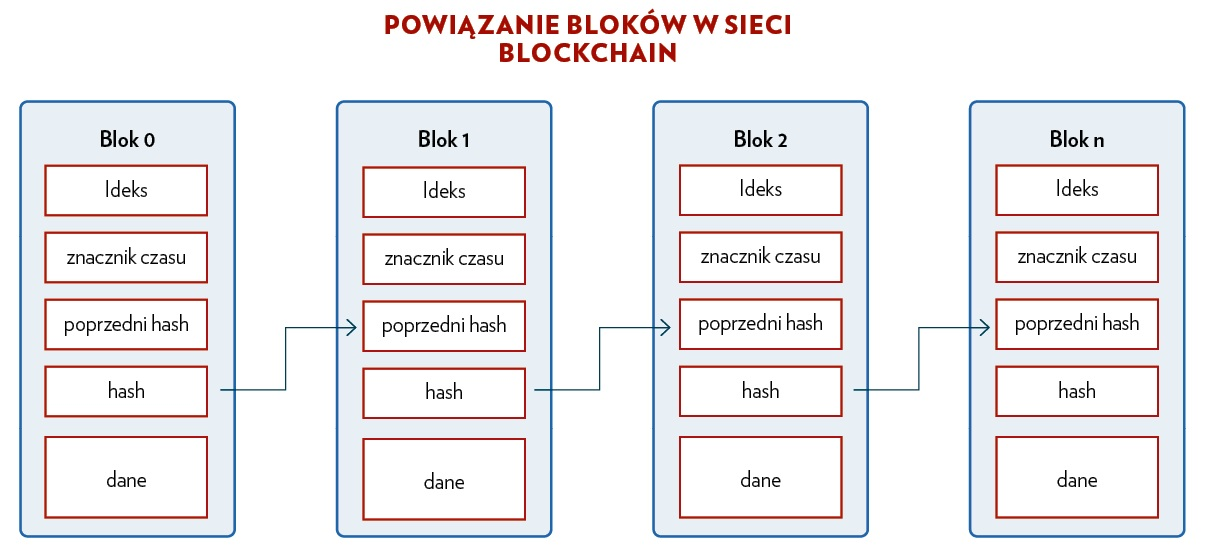
\includegraphics[width=\textwidth]{images/łańcuch_bloków.jpg}
	\caption {Łańcuch bloków.}
\end {figure}

Na rysunku 2.1 ukazany jest schemat łańcucha bloków. Jak widać dane przechowywane są w blokach, a bloki połączone są za pomocą wskaźników na hash poprzedniego bloku. Taka budowa stanowi zabezpieczenie łańcucha bloków przed modyfikacją lub usunięciem danych. Modyfikacja dowolnego bloku w sieci jest widoczna i łatwa do zweryfikowania. Wystarczy policzyć od początku hash dla każdego bloku i porównać z polem następnego bloku, które przechowuje poprzedni hash.

\subsection{Sieci Peer to Peer}

Zmodyfikowanie łańcucha bloków jest trudne, lecz nie jest niemożliwe. Wymaga jedynie wystarczająco dużej mocy obliczeniowej. Dodatkowo zamiast modyfikować łańcuch, można przejąć urządzenie, na którym uruchomiony jest łańcuch bloków, co daje możliwość zakłócenia pracy systemu opartego na działaniu łańcucha.

Twórcy Bitcoina rozwiązali podane problemy wykorzystując zdecentralizowaną sieć Peer-to-Peer. Sieć Peer-to-Peer składa się z węzłów, które komunikują się ze sobą, bez centralnego serwera. Jeżeli węzły chcą się ze sobą skontaktować, to wysyłają dane bezpośrednio do siebie. Takie rozwiązanie pozwala zwiększyć bezpieczeństwo sieci, ponieważ trudniej jest przejąć kontrolę nad wieloma maszynami tworzącymi całą sieć, niż nad centralnym systemem obsługującym działanie tej sieci. Dodatkowo P2P zapewnia zabezpieczenie danych zgromadzonych w sieci, przed usunięciem, ponieważ każde urządzenie przechowuje swoje egzemplarze danych, które można traktować jako kopie zapasowe. Dystrybucja sieci na całym świecie zabezpiecza sieć przed cenzurowaniem, z czego korzysta Bitcoin i inne kryptowaluty.

Peer-to-Peer jest przykładem ciekawego zastosowania architektury klient-serwer. Architektura klient serwer polega na podzieleniu systemu na stronę kliencką, która zajmuje się wysłaniem żądań do serwera, oraz na stronę serwerową, której zadaniem jest odpowiadanie na żądania, przechowywanie danych i operowanie na tych danych. W sieci P2P węzeł pełni role zarówno serwera, jak i klienta. Przykładowo węzeł może żądać przesłania danych od innego węzła, a także odpowiedzieć na żądanie innego węzła.

\subsection{Konsensus}

Konsensus w sieci Blockchain oznacza, że każdy z jej uczestników zgadza się na stan danych przechowywanych w sieci. Każda aktywność zmieniająca stan przechowywanych danych powinna być autoryzowana, aby zapewnić bezpieczeństwo i spójność sieci. Konsensus pozwala na wprowadzenie do sieci zestawu reguł, według których działa cała sieć. Takie działanie pozwala na zweryfikowanie zaufanego źródła i wykluczenie wpływu węzłów dziłających na szkodę sieci. W kryptowalutach najczęściej wykorzystywane algorytmy konsensusu to Proof of Work i Proof of Stake. Natommiast Proof of Authority dotyczy rozwiązań prywatnych.

\subsubsection{Proof of Work}

Proof of work to popularny w kryptowalucie Bitcoin algorytm uzyskiwania konsensusu. Algorytm ten wykorzystywany jest podczas tworzenia nowego bloku. Nowy blok wysyłany jest do wszystkich węzłów w sieci, które w celu dodania bloku do swojego łańcucha muszą zostać zatwierdzone. Na tym etapie algorytmu mamy do czynienia z popularnymi "koparkami" Bitcoinów. Aby blok został zatwierdzony węzeł musi wykonać pracę, czyli dokonać wkładu mocy obliczeniowej. Moc obliczeniowa wykorzystywana jest do rozwiązania zagadki matematycznej. Praca ta wykonywana jest przez węzeł i jest określana jako mining (pol. wydobywanie).Ten węzeł, który jako pierwszy rozwiąże zagadke, otrzyma nagrodę w postaci określonej ilości środków, w kryptowalucie Bitcoin. W typowych rozwiązaniach dla Bitocoinu poziom trudności dodania nowego bloku jest tak skonstruowany, aby nowe bloki były dodawane, w odstępach około 10 minutowych\cite{pow-bitcoin}.

Takie rozwiązanie premiuje węzły, o większej mocy obliczeniowej. Dlatego w celu utrzymania spójności danych należy przeprowadzać synchronizację węzłów. Synchronizacja przebiega nastepująco: każdy węzeł rozsyła do całej sieci swój łańcuch, węzły porównują długość swojego łańcucha z nadesłanym łańcuchem i w węźle zapisywany jest dłuższy łańcuch.

Proof of work to rozwiązanie towarzyszące architekturze Blockchain, od momentu jej powstania. Bitcoin poza dokonywaniem transakcji, pozwala na zarabianie poprzez tworzenie tzw. węzłów górniczych. Węzeł górniczy zajmuje się realizacją algorytmu Proof of Work, co oznacza rozwiązywanie zagadki matematycznej. Fizycznie jest to urządzenie, ze specjalistycznymi podzespołami i oprogramowaniem, które pozwala na uzyskanie wysokiej efektywności w wydobywaniu Bitcoina \cite{nodes}. Głównym problemem tego rozwiązania jest zużycie energii elektrycznej. W roku 2017 zużycie energii elektrycznej, przez wydobywanie Bitcoina było większe, niż w 159 krajach na świecie \cite{elctricity-bitcoin}. W 2019 naukowcy z University of Cambridge stworzyli specjalny indeks (CBECI), ukazujący dane dotyczące zużycia energii elektrycznej, przez Bitcoin'a \cite{CBECI}.

W tym algorytmie czynnik wkładu fizycznych zasobów, jest głównym motywatorem do uczciwego postępowania. Jednakże głownym czynnikiem sprawiającym, że ten algorytm działa jest pewność, że ponad 50\% uczestników sieci działa uczciwie. Ogrom inwestowanych zasobów wpływa na bezpieczeństwo sieci. Duża zdecentralizowana sieć Blockchain dysponuje ogromną mocą obliczeniową, na jej moc składa się moc wszystkich węzłów w sieci. Węzły różnią się mocą obliczeniową, natomiast decentralizacja sieci sprawia, że żaden z węzłów nie może przejąć kontroli nad całą siecią. Im większa decentralizacja tym bardziej zmniejsza się wpływ pojedynczego węzła na całą sieć. Co innego, gdy do sieci dołączona zostanie grupa węzłów, które będą stanowiły 51\% mocy obliczeniowej sieci oraz będą ze sobą współpracowały, działając na szkodę sieci. Taki scenariusz nazywany jest atakiem 51\%. Dysponując 51\% mocy obliczeniowej sieci, można bez wiedzy uczciwych uczestników, w szybszy sposób dodawać nowe bloki, co prowadzi do przejęcia obsługi dodawania zawartości, przez szkodliwych uczestników siec\cite{atack51}i.

W przypadku algorytmu Proof of Work atak 51\% jest bardzo rzadkim zjawiskiem, gdyż jest on bardzo drogi. Atak ten może być opłacalny jedynie wtedy, gdy atakujący chce zdestabilizować sieć. W przypadku Bitcoin'a destabilizacja sieci nie ma większego sensu, ponieważ dysponując taką mocą obliczeniową można uzyskać ogromne przychody z kopania Bitcoin'a, dodatkowo uzyskanie takiej mocy obliczeniowej w rozrastających się sieciach Blockchain dla Bitcoin'u jest na tyle drogie, że w teorii jest uznawane za nieosiągalne. Z tego powodu, w przypadku sieci Blockchain, bardzo ważne jest zadbanie o jak największe rozproszenie węzłów w sieci P2P.

\subsubsection{Proof of Stake}

Proof of Stake to kolejny algorytm używany do osiągania konsensusu w sieciach Blockchain. Jego największe zalety, to rozwiązanie problemu wykorzystania ogromnych ilości zasobów energii elektrycznej przez algorytm Proof of Work.

Działanie algorytmu Proof of Stake polega na wybieraniu spośród dostępnych węzłów sieci Blockchain walidatora. Walidator to węzeł, którego zadaniem jest weryfikacja poprawności bloku dołączanego do łańcucha. Wybór walidatora może się odbywać na różne sposoby, od całkowicie losowego wyboru, po wybór z uwzględnieniem czynników takich jak np. wiek stawki węzła, wysokość stawki. Stawka to zablokowane na koncie danego węzła jednostki waluty (kryptowaluty). Stawka jest wymagana, aby węzeł mógł uczestniczyć w losowaniu.

W przypadku algorytmu Proof of Stake głównym motywatorem uczciwego uczestnictwa w sieci jest możliwość utracenia części stawki. W przypadku wykrycia przez sieć nieprawidłowości w bloku dodanym przez konkretny węzeł, traci on określoną część stawki.

Proof of Stake jest o wiele bardziej ekologiczny, jeśli chodzi o zużycie energii elektrycznej, niż Proof of Work. Oznacza to, że sieć jest dostępna dla większej ilości urządzeń, co wpływa na zwiększenie rozproszenia sieci. W Proof of Stake głównym czynnikiem determinującym moc sieci jest zgromadzony w niej wkład finansowy w postaci stawek. W przypadku tego algorytmu również występuje problem ataku 51\%, jednakże tym razem atakujący musi dysponować odpowiednią ilością środków płatniczych, a dokładnie musi włożyć 51\% ogólnej stawki, co w przypadku Bitcoin'a jest mało prawdopodobne.

\subsubsection{Proof of Authority}
Proof of Authority to rozwiązanie skłaniające się ku mniej zdecentralizowanym systemom, które są tworzone na prywatne potrzeby i wymagających dużej przepustowości. Proof of Authority jest w swoim działaniu nieco zbliżony do Proof of Stake. Zamiast stawki podanej w jednostkach odpowiedniej waluty, w PoA używana jest reputacja walidatora. Prowadzi to do skonstruowania sieci, w której uczestniczą tylko zaufani walidatorzy. Uzyskanie statusu walidatora wiąże się z dużym nakładem pracy, w celu spełnienia kryteriów i uzyskania odpowiednio wysokiej reputacji. Podczas projektowania takiego systemu należy zwrócić szczególna uwagę, na stworzenie kryteriów o wysokiej trudności do spełnienia, aby wykluczyć węzły o szkodliwym działaniu.

Trudność uzyskania statusu walidatora bardzo mocno wpływa na stopień zdecentralizowania. Decentralizacja porównywalna z rozwiązaniem Proof of Stake jest niemożliwa do osiągnięcia.
Niski stopień decentralizacji wymaga pełnego zaufania do walidatorów, co może stanowić słaby punkt systemu, gdy zaufany walidator zostanie przekupiony i dokona szkodliwej manipulacji na zawartości systemu.

Algorytm Proof of Authority świetnie sprawdza się w prywatnych sieciach Blockchain, gdy ważna jest wysoka przepustowość łącza. Jednakże należy pamiętać o odpowiednim doborze walidatorów.

\subsection{Funkcja skrótu}

Funkcje skrótu w systemach informatycznych pełnią rolę zabezpieczenia integralności danych. Zabezpieczenie danych polega na wykryciu modyfikacji. Matematyczna definicja funkcji skrótu h to odwzorowanie wiadomości m o dowolnej , skończonej długości, w ciąg bitów o określonej, stałej długości n \cite{hash}:

\begin{equation}
h:\left \{0, 1\right \}^{*}\rightarrow \left \{0, 1\right \}^{n}, gdzie: \left \{0, 1\right \}^{*}=\bigcup_{i\in  N}\left \{0, 1\right \}^{i}, N = \left \{0, 1, ...\right \}, n \in N
\end{equation}

Funkcja skrótu (hash) cechuje się wysoką podatnością na zmiany. Zmiana jednego bitu w danych wejściowych powoduje otrzymanie zupełnie innych wyników. \newline
Przykładowo dla ciągu znaków hash0, dla funkcji skrótu SHA256 wynikiem jest ciąg znaków
\newline 6ac73742db534bebccc9af1453c5637ee5bb5d7c9628ec2f26cf9777c89e96d8. Natomiast zmieniając ciąg znaków na hash1, otrzymanym wynikiem jest \newline af316ecb91a8ee7ae99210702b2d4758f30cdde3bf61e3d8e787d74681f90a6. Przykład obrazuje jak na wynikowy ciąg znaków wpływa zmiana jednego symbolu na wejściu.

Głównymi cechami funkcji skrótu są:
\begin{itemize}
	\item Nieodwracalność - na podstawie otrzymanego wyniku nie można bezpośrednio odtworzyć danych.
	\item Bezkolizyjność - nie istnieją dwa różne ciągi znaków, które dają ten sam wynik.
\end{itemize}

Znalezienie danych wejściowych dla funkcji skrótu jest zadaniem wymagającym dużego nakładu mocy obliczeniowej. Dane można uzyskać losując wejściowy ciąg znaków i hashując go, a następnie porównując otrzymany hash z hashem, który ma być rozszyfrowany. Jest to tak zwany atak brutalny (ang. brute force).

Popularnym zastosowaniem funkcji skrótu jest podpis cyfrowy. Podpis cyfrowy to zaszyfrowany hash, wygenerowany na podstawie danych potrzebnych do podpisu. Głównym zaletą wykorzystania hash'owania w podpisie cyfrowym jest szybkość. Hashowanie wiadomości jest szybsze od szyfrowania, a zaszyfrować wystarczy sam ciąg znaków o stosunkowo małej długości, w porównaniu do tekstu wiadomości.

Funkcje skrótu można spotkać w bazach danych. Hasła są przykładem informacji, które w bazie danych są przechowywane w postaci funkcji skrótu. Takie rozwiązanie zabezpiecza hasła, w przypadku wycieku danych.

\subsection{Smart kontrakty}

Wraz z powstaniem kryptowaluty Ethereum do architektury Blockchain została dodana nowa funkcja. Dodano tak zwane Smart Kontrakty, które pozwalają na zaprogramowanie i uruchomienie kodu w sieci Blockchain. Takie programy można stosować, w celu kontrolowania sieci poprzez zdefiniowanie zestawu reguł dla sieci. Zdefiniowanie zestawu reguł pozwala na zwiększenie zaufania w sieci, a także automatyzację niektórych procesów.

Smart kontrakty pozwalają na tworzenie aplikacji, których podstawą jest Blockchain. Przykładem środowiska pozwalającego na tworzenie takich programów jest język Solidity, który został stworzony dla sieci Ethereum\cite{smart-contract}. 

\newpage

\section{Technologia Blockchain na rynku}

\subsection{Kryptowaluty}

Kryptowaluta to cyfrowy środek płatniczy. W przeciwieństwie do tradycyjnych walut, kryptowaluty nie są kontrolowane przez bank centralny. Środki płatnicze w kryptowalucie znajdują się w rozproszonej, po całym świecie sieci. Każda transakcja w tym środowisku jest zapisywana we współdzielonym rejestrze. Rejestr pozwala na ustalenie ile środków w danej kryptowalucie jest na koncie danego uczestnika sieci. Podstawą działania kryptowalut jest Blockchain. To Blockchain odpowiada za tworzenie rejestru transakcji, zabezpieczenie danych przed modyfikacją, współdzielenie danych i uzyskanie konsensusu. Przykładem takich kryptowalut są Bitcoin i Ethereum.

\subsection{Finanse}

Dynamiczny rozwój technologii zapoczątkował rozwój innych branż, w tym sektora finansów. Powstała osobna gałąź tego sektora o nazwie FinTech. FinTech zajmuje się opracowywaniem i wdrażaniem nowych technologii do systemów finansowych na całym świecie. Korzyści płynące z unowocześnienia sektora finansów mogą skupiają się głównie na zwiększeniu szybkości transakcji przez brak pośredników, zmniejszeniu kosztów przepływu transakcji i zwiększenie bezpieczeństwa. FinTech zajmuje się między innymi szukaniem zastosowań dla technologii Blockchain. Jako przykład rozwijania technologii blockchain przez FinTech może posłużyć przykład trwałego nośnika wdrożonego przez PKO Bank Polski. Trwały nośnik pozwala na dostarczanie klientom banku prywatnych dokumentów w formie cyfrowej \cite{PKO}. Twórcy tego rozwiązania zastosowali również mechanizm Smart Kontraktów. Smart Kontrakty są wykorzystywane do zautomatyzowania procesu egzekwowania umów ubezpieczeniowych\cite{PKO-SMART}. Pozwala to na zmniejszenie uczestnictwa osób trzecich i redukcję kosztów.

\subsection{Internet of Things}

Internet of Things to technologia pozwalająca na łączenie ze sobą wielu urządzeń. Tak skonstruowane sieci znajdują swoje przeznaczenie w systemach czasu rzeczywistego w przemyśle, bądź w inteligentnym domu. IoT wykorzystuje serwery internetowe, do przechowywania i pobierania danych. Blockchain w usługach IoT pomaga zabezpieczyć serwery z danymi, poprzez ich decentralizację.

\newpage

\section{Przegląd istniejących rozwiązań e-votingu}
\section{System estoński}
Przykładem regularnego wykorzystania e-votingu jest Estonia. Estonia jest krajem, który pierwszy udostępnił możliwość głosowania elektronicznego w wyborach lokalnych, na szczeblu krajowym. W pierwszych wyborach wzięło udział około 1\% wyborców. Od roku 2005 w Estonii postępował rozwój systemów e-votingu. Wraz z następnymi wyborami zwiększała się liczba uczestników. W roku 2019 liczba wyborców, którzy skorzystali z e-votingu wyniosła 43,8\% wyborców.

Na system e-votingu w Estonii składa się kilka mniejszych rozwiązań, które można wylistować w następujący sposób:
\begin{itemize}

\item Identyfikacja za pomocą karty e-obywatela lub profilu e-obywatela w telefonie.

\item Architektura rozwiązania pozwala na wysłanie wielu głosów, a głosem wiążącym jest zawsze głos finalny.

\item Serwery wykorzystywane podczas głosowania są pod szczególną ochroną i nie można uzyskać do nich dostępu z bezpośrednio z internetu (zabezpieczenie firewallem).

\item Wykorzystywanie prywatnych kluczy i narzędzi kryptograficznych w celu zabezpieczenia dostępu do danych. Wykorzystywanie standardu SSL.
\end{itemize}

\subsection{Przegląd rozwiązania}
Przebieg całego procesu wyborczego w Estonii można podzielić na kilka etapów:
\begin{itemize}
\item ogłoszenie wyborów;
\item zarejestrowanie kandydatów;
\item przygotowanie list wyborczych;
\item głosowanie;
\item liczenie głosów;
\item ogłoszenie wyników;
\end{itemize}

Wsparcie e-votingu (w Estonii określanego i-votingiem) obejmuje ostatnie trzy etapy procesu wyborczego.

\begin{figure}[h]
	\centering
	\includegraphics[width=\textwidth]{images/Dziedzina systemu estońskiego}
	\caption{Moduły systemu i-votingu.}
\end {figure}
\newpage

W skład systemu głosowania wchodzą bazy danych przechowujące:
\begin{itemize}
\item listę osób uprawnionych do głosowania;
\item listę okręgów wyborczych;
\item listę kandydatów lub opcji wyborczych;
\item listę e-wyborców (i-voters);
\end{itemize}

Dostarczenie odpowiednich danych do systemu pozwala na walidację wyborcy, zgłoszenie przez
niego głosu oraz zapisanie wyborcy, w bazie danych odpowiedzialnej za przechowanie listy e-wyborców. W skład logiki systemu wchodzą mechanizmy generujące wyniki. Wyniki e-votingu są scalane z wynikami wyborów tradycyjnych, przy czym scalanie nie pozwala na podwójne zliczanie głosu oddanego tradycyjnie i elektronicznie.

\begin{figure}[h]
	\centering
	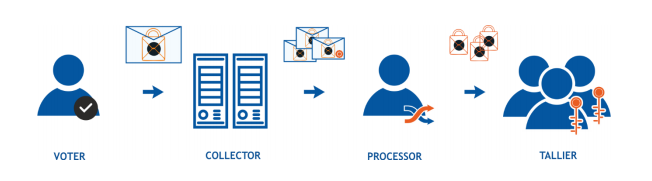
\includegraphics[width=\textwidth]{images/Główne częsci systemu estońskiego.png}
	\caption{Proces wyborczy.}
\end {figure}

Główne części systemu:
\begin{itemize}
\item Voter (dalej nazywany wyborcą) - za pośrednictwem aplikacji klienckiej (która w systemie estońskim jest aplikacją desktopową pobieraną przed wyborami) szyfruje i potwierdza swoim podpisem elektronicznym głos, który następnie wysyłany jest do Kolektora.
\item Collector (dalej nazywany Kolektorem) - to aplikacja serwerowa wyposażona w logikę pozwalającą na utworzenie głosu. Aplikacja waliduje dane wprowadzone przez wyborcę i elektronicznie podpisuje dane, które następnie przesyła do Procesora.
\item Processor (dalej nazywany Procesorem) - zajmuje się przetwarzaniem głosów. Sprawdza poprawność danych otrzymanych z Kolektora, wraz z podpisem elektronicznym. Usuwa głosy, które się powtarzają, zarówno głosy oddane elektronicznie, jak i te oddane w lokalach wyborczych. Sortuje głosy według okręgów wyborczych i usuwa z nich podpis elektroniczny, w celu anonimizacji głosu. Tak przetworzone głosy są mieszane według odpowiedniego algorytmu i wysyłane do Licznika.
\item Tallier (dalej nazywany Licznikiem) - rolą licznika jest odebranie głosu od Procesora, otwarcie go i dodanie przyporządkowanie do odpowiedniego wyniku.
\end{itemize}

\section{Aplikacja internetowa Votex}

\section{Evoting w Walnych Zgromadzeniach}

Krajowy Depozyt Papierów Wartościowych to instytucja finansowa, której zadaniem jest nadzorowanie i prowadzenie rejestracji obrotu instrumentami finansowymi w Polsce. KDPW pełni również rolę depozytu papierów wartościowych. KDPW jest spółką akcyjną, której współwłaścicielami są akcjonariusze - państwo (Skarb Państwa) i państwowe spółki finansowe (Giełda Papierów Wartościowych, Narodowy Bank Polski).

Walne Zgromadzenie to organ mający najwyższe uprawnienia w spółce akcyjnej. Walne Zgromadzenie pozwala akcjonariuszom na zarządzanie spółką. Podczas Walnego Zgromadzenia podejmuje się uchwały dotyczące spółki akcyjnej.

Krajowy Depozyt Papierów Wartościowych udostępnia swoim akcjonariuszom aplikacje e-voting oraz Walne Zgromadzenia, które przenoszą proces przeprowadzania Walnego Zgromadzenia do internetu. Zgodnie z art. 402 Kodeksu Spółek Handlowych \cite{sp-han}, Walne Zgromadzenie zwoływane jest przez ogłoszenie go, co najmniej trzy tygodnie przed zaplanowanym terminem. W celu zwołania Walnego Zgromadzenia w aplikacji Evoting i Walne Zgromadzenia należy zarejestrować Walne Zgromadzenie. KDPW przesyła ogłoszenie, o Walnym Zgromadzeniu do jego uczestników. Wymiana informacji odbywa się drogą elektroniczną.
Uczestnicy tworzą listę osób uprawnionych do udziału w Walnym Zgromadzeniu, która jest przesyłana do KDPW. KDPW generuje wykaz osób uprawnionych do uczestnictwa w Walnym Zgromadzeniu, a następnie dostarcza informacje o uczestnictwie w Walnym Zgromadzeniu indywidualnie, dla każdego uczestnika. Każdy uczestnik otrzymuje również kod autoryzacyjny, który wykorzystywany jest do potwierdzenia tożsamości uczestnika, w celu przyznania uprawnień do uczestnictwa w Walnym Zgromadzeniu. Przyznanie uprawnień jest równoznaczne z potwierdzeniem obecności na Walnym Zgromadzeniu i udostępnieniu uczestnikowi interfejsu do głosowania \cite{eVoting-dzialanie}.

Za zapewnienie nieodwracalności wykonanych akcji i ogólnego bezpieczeństwa danych, w aplikacjach eVoting i Walne Zgromadzenia jest odpowiedzialny Blockchain.

\chapter{Wymagania systemu i wykorzystane narzędzia}
W tym rozdziale sformułowano i omówiono wymagania funkcjonalne i niefunkcjonalne. Dodatkowo przedstawiono przypadki użycia i aktorów systemu. Na koniec opisane zostały technologie i narzędzia wykorzystane podczas tworzenia systemu.

\section {Wymagania funkcjonalne}

W tej sekcji umieszczono wszystkie funkcjonalności i części systemu. Do głównych części systemu należą: aplikacja internetowa wyborcy, aplikacja internetowa administratora wyborów,
serwis udostępniający REST (Representational State Transfer) API i serwery sieci Blockchain. Do wymagań funkcjonalnych systemu należą:

\begin{itemize}
	\item Hasła przechowywane w bazie danych są szyfrowane za pomocą funkcji skrótu SHA256,
	\item Dostęp do zasobów wyborcy i administratora odbywa się poprzez dwie inne aplikacje internetowe,
	\item Komunikacja pomiędzy aplikacjami przeglądarkowymi, a API odbywa się z wykorzystaniem konwencji REST API,
	\item Dostęp do punktów końcowych API (endpointów) jest zabezpieczony za pomocą JWT (Json Web Token) oraz uwierzytelnienia na podstawie roli (Role Based Authentication),
	\item Dostęp do zasobów posiadają tylko zalogowani użytkownicy,
	\item Za bezpieczne przechowywanie głosów odpowiadają sieci Blockchain,
	\item Każdy węzeł sieci Blockchain to indywidualny program umożliwiający konfigurację sieci,
	\item Dla każdych wyborów konfigurowana jest indywidualna sieć Blockchain,
	\item Dostęp do sieci Blockchain uzyskiwany jest za pomocą serwisu,
	\item Komunikacja pomiędzy serwisem, a siecią Blockchain odbywa się z udziałem jednego węzła, który odbiera informacje i rozsyła po całej sieci,
	\item Konsensus w sieci może być uzyskiwany z wykorzystaniem algorytmu Proof of Work lub Proof of Authority.
\end{itemize}

\section {Wymagania niefunkcjonalne}

Wymagania niefunkcjonalne definiują jakość usług dostarczanych przez system. W systemie e-votingu ważnymi elementami są bezpieczeństwo i czytelność procedury głosowania. Dlatego w celu uściślenia oczekiwań jakościowych systemu sformułowano następujące wymagania niefunkcjonalne:

\begin{itemize}
	\item Dane logowania użytkownika są zabezpieczone,
	\item Dane logowania administratora są zabezpieczone,
	\item Przechowywane głosy są zabezpieczone przed modyfikacją,
	\item Przejrzyste treści na stronie wyborcy,
	\item Czytelna i łatwa w obsłudze procedura wyborcza na stronie wyborcy,
	\item Przejrzyste treści na stronie administratora wyborów,
	\item Czytelna i łatwa w obsłudze konfiguracja wyborów,
	\item Aplikacje internetowe wyborcy i administratora działają na najpopularniejszych przeglądarkach internetowych.
	\item Czas liczenia głosów jest zdeterminowany.
\end{itemize}
\newpage

\section{Diagramy przypadków użycia}

W systemie można wyróżnić dwóch aktorów. W tym podrozdziale zostały przedstawione i omówione diagramy przypadków użycia dla aktorów.

\begin{figure}[h]
	\centering
	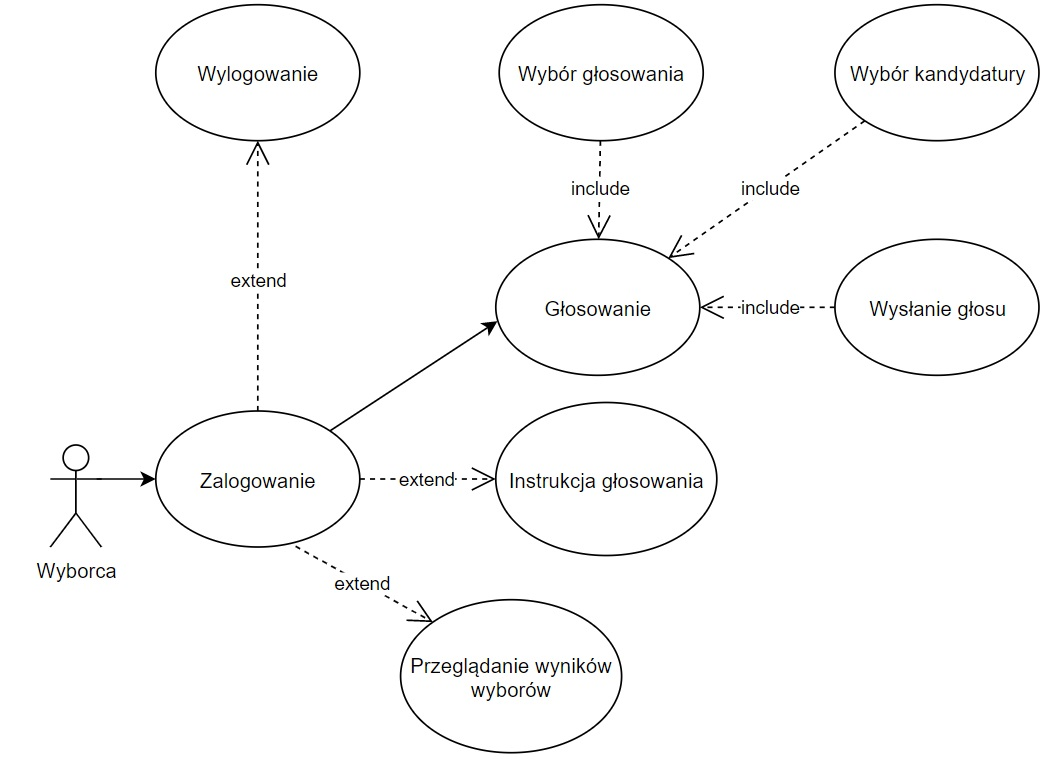
\includegraphics[width=\textwidth]{images/user_use_case.jpg}
	\caption{Diagram przypadków użycia użytkownika.}
\end {figure}

\begin{figure}[h]
	\centering
	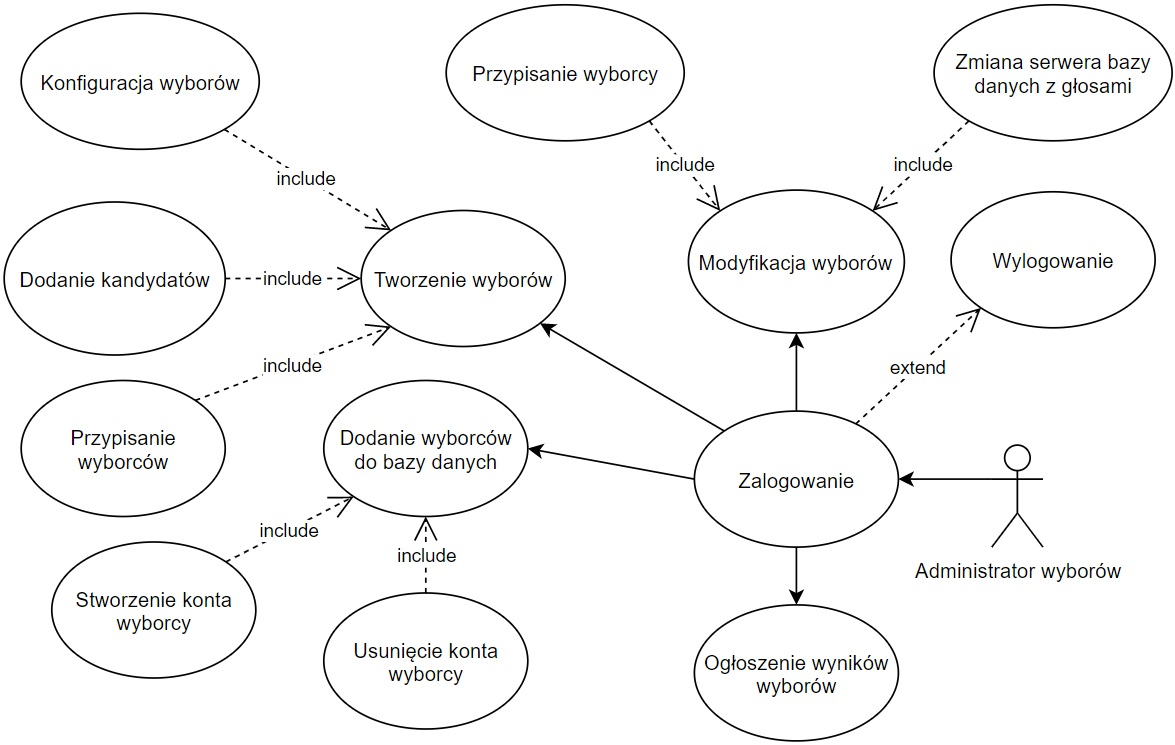
\includegraphics[width=\textwidth]{images/admin_use_case.jpg}
	\caption{Diagram przypadków użycia administratora.}
\end {figure}

\newpage
\section {Wykorzystane narzędzia i technologie}

System e-votingu jest składa się z wielu modułów, których stworzenie obejmuje różne dziedziny programowania. W systemie są elementy odpowiedzialne za interfejs użytkownika, aplikację serwerową i bazę danych. Każdy z tych rodzajów oprogramowania wymaga innego podejścia. Są to popularne dziedziny programowania, dlatego znalezienie rozwiązań nie stanowi problemu. W tej sekcji przedstawiono wykorzystane narzędzia i technologie, a także ich zastosowania w projekcie.

\subsection{Interfejs użytkownika}

W celu stworzenia rozbudowanego interfejsu użytkownika wykorzystano bibliotekę javascript-ową - ReactJs. React pozwala na tworzenie aplikacji internetowych z wykorzystaniem języków javascript, html i css. Takie podejście do tworzenia aplikacji określane jest jako SPA (Single Page Application), taka aplikacja posiada jeden plik html, którego zawartość jest dynamicznie generowana w trakcie działania aplikacji. Podejście SPA pozwala na zredukowanie liczby zasobów potrzebnych do generowania strony, poprzez wykorzystanie tylko jednego pliku html. Strona typu SPA działa płynnie, ponieważ nie wymaga ona ładowania szablonów z plików html. Ważną cechą ReactJs jest podejście do interfejsu użytkownika, jak do grupy komponentów. Komponent może być dowolnym elementem interfejsu, od paska nawigacji do przycisku. Każdy komponent posiada swój stan, czyli zestaw zmiennych kontrolujących jego funkcjonalności. Takie podejście pozwala na tworzenie uniwersalnych komponentów, które można wykorzystywać w wielu miejscach aplikacji.

Biblioteka ReactJs to bardzo rozbudowane narzędzie, które dzięki swojej popularności posiada wiele dodatkowych narzędzi współpracujących z całym środowiskiem ReactJs. Przykładem takiego dodatku jest biblioteka Redux, która pozwala na zarządzanie stanem aplikacji. Redux pozwala przenieść stan z komponentu do osobnego kontekstu. Takie rozwiązanie pozwala na umieszczenie tych części stanu aplikacji, które odnoszą się do różnych komponentów w jednym miejscu. Przykładowo stan informujący o zalogowaniu do aplikacji powinien być dostępny dla całej aplikacji. Przeniesienie tego stanu do osobnego kontekstu pozwala na zdefiniowanie go w jednym miejscu i dostarczenie do komponentów, które wymagają tego stanu. W projekcie wykorzystano opartą na Redux, bibliotekę Redux-Toolkit. Głównym argumentem za wykorzystaniem Redux-Toolkit jest mniejsza objętość kodu, która powstaje do uzyskania rozwiązania.

Podstawowym narzędziem odpowiedzialnym za wygląd interfejsu aplikacji internetowej są kaskadowe arkusze stylów, czyli popularny CSS (Cascade Style Sheets). Język css jest jedynym językiem odpowiedzialnym za stylowanie wyglądu, który jest rozumiany przez przeglądarkę. Jednakże istnieją rozwiązania, które pozwalają na wprowadzenie nowej składni z zachowaniem kompatybilności z danym środowiskiem uruchomieniowym (w tym przypadku z przeglądarką). Są to tzw. preprocesory. Preprocesor pozwala na przetworzenie kodu źródłowego na określony kod wyjściowy. Przykładem preprocesora języka CSS, który został wykorzystany w projekcie jest Sass. Sass dostarcza funkcjonalności, które nie są dostępne w języku CSS. Przykładowo Sass pozwala na zagnieżdżanie instrukcji, deklarowanie i wywoływanie zmiennych oraz tzw. mixins, które pozwalają na zadeklarowanie powtarzających się fragmentów kodu w jednym miejscu i ich wywoływanie bez konieczności przepisywania kodu. Sass pozwala na lepsze wykorzystanie dobrych praktyk programowania, takich jak nie powtarzanie kodu i ogólna poprawa jakości kodu.

Jak już wspomniano w tej sekcji ReactJs jest popularną biblioteką, co owocuje dużą ilością rozszerzeń i dodatków. Dodatki obejmują również stylowanie aplikacji. W projekcie została wykorzystana biblioteka Material-ui, która dostarcza gotowe zestawy komponentów i narzędzia do ich stylowania. Zaletą tego rozwiązania jest wykorzystywanie komponentów, które stworzono z wykorzystaniem dobrych praktyk tworzenia interfejsu.

Aplikacje internetowe często wymagają komunikacji z zewnętrznym serwer, w celu pobrania lub wysłania odpowiednich zasobów. Takie działanie to przykład architektury klient-serwer. Istnieje wiele rozwiązań, które pozwalają na wysyłanie żądań w standardzie HTTP. W projekcie wykorzystano javascript-ową bibliotekę Axios. Biblioteka dostarcza wszelkich mechanizmów do wysyłania żądań HTTP, a jej wielką zaletą jest łatwość obsługi.

Javascript to język programowania, który świetnie sprawdza się w środowisku aplikacji przeglądarkowych. Język umożliwia wieloaspektowe podejście do program. Można pisać programy z podejściem deklaratywnym lub obiektowym. Javascript spełnia najważniejsza standardy, dla nowoczesnych języków programowania, o czym świadczyć może ogromna popularność tego języka. Jednakże niektóre właściwości tego języka mogą utrudniać tworzenie oprogramowania. Przykładem jest typowanie dynamiczne.W Javascript każda zmienna nie ma przypisanego typu na stałe. Takie rozwiązanie ma swoje wady i zalety, jednak programista powinien mieć wybór, kiedy użyć zmiennej typowanej dynamicznie, a kiedy nie. Rozwiązaniem tego problemu jest język Typescript. Typescript jest nadzbiorem javascript co oznacza, że dostarcza on wszystkie funkcje Javascriptu i jednocześnie rozszerza go o nowe. W Typescript można deklarować zmienne z określonym typem, a także używać typu any. Typ any określa zmienne, które mogą być typowane dynamicznie. Język Typescript dostarcza również możliwość definiowania własnych typów. W projekcie, w celu uniknięcia problemów związanych z dynamicznym typowaniem wykorzystano język Typescript.

\subsection{Serwer}
Za stronę serwerową aplikacji odpowiada silnik NodeJs. NodeJs pozwala na tworzenie aplikacji w Javascript, poza środowiskiem przeglądarkowym. Silnik stanowi również rozbudowane narzędzie pozwalające na tworzenie REST API. Zaletą NodeJs jest ogromna popularność, co jest zauważalne podczas szukania rozwiązań na portalu Stackoverflow. Popularność silnika przekłada się również na jego bogatą dokumentację i dodatkowe biblioteki, które usprawniają elementy tworzenie oprogramowania.

ExpressJs to biblioteka działająca na silniku NodeJs, która została wykorzystana w projekcie do tworzenia REST API i węzłów sieci Blockchain. ExpressJs dostarcza podstawowe narzędzia do tworzenia REST API, takie jak endpointy (punkty końcowe serwera) pozwalające na obsługiwanie żądań HTTP. Zaletą biblioteki ExpressJs jest kompatybilność z wieloma innymi bibliotekami przeznaczonymi dla silnika NodeJs.

Prisma to jedna z bibliotek NodeJs, które są odpowiedzialne za obsługę bazy danych. Prisma dostarcza mechanizm ORM (Object Relational Mapping), czyli możliwość odwzorowania relacyjnej bazy danych, na obiekty. Prisma generuje moduły odpowiedzialne za obsługę bazy danych i dostarcza je programiście. Takie rozwiązanie pozwala na utrzymanie całości aplikacji w jednym języku programowania, ponieważ nie wymaga korzystania z języka SQL, w celu zarządzania bazą danych z poziomu aplikacji. Prisma pozwala oddzielić implementację bazy danych, od innych funkcjonalności aplikacji.

\subsection {Baza danych}

Wykorzystana baza danych to SQLite. Baza danych znajduje się w pliku i jest umieszczona na serwerze wraz z REST API. SQLite to szybki, mały i łatwy w konfiguracji silnik baz danych. Jest to świetny silnik do prototypowania i tworzenia małych, a zarazem przenośnych baz danych.

Silnik SQLite można obsługiwać z poziomu konsoli lub za pomocą specjalnej aplikacji, która dostarcza interfejs graficzny prezentujący zawartość bazy danych. W projekcie wykorzystano aplikację SQLiteStudio, która pozwala na połączenie się z bazą danych, w celu zarządzania nią. SQLiteStudio pozwala na tworzenie tabel, dodawanie zawartości, usuwanie danych i przeszukiwanie bazy danych. Aplikacja pozwala również na pisanie własnych zapytań w języku SQL. Tego rodzaju aplikacje są przydatne podczas tworzenie tabel w bazie danych i testowania aplikacji.

\subsection{Testowanie}

Testowanie strony serwerowej systemu odbywało się przez aplikację Postman, która pozwala na wysyłanie żądań HTTP każdego rodzaju. W aplikacji można skonfigurować żądanie HTTP, tak aby zasymulować odpowiednie scenariusze żądania. Pozwala to przetestować działanie wszystkich funkcjonalności API.

Testowanie aplikacji w środowisku lokalnym pozwala odpowiedzieć na pytanie, czy całość komponentów działa w kontrolowanym środowisku. Natomiast przeniesienie aplikacji do sieci pozwala na przetestowanie wydajności aplikacji. W projekcie, w celu udostępnienia aplikacji w internecie wykorzsytano serwisy Netlify oraz Heroku. Netlify pozwala na udostępnienie aplikacji internetowej, pod adresem generowanym przez serwis. Heroku zajmuje się uruchomieniem aplikacji serwerowej, która również dostępna jest w sieci pod odpowiednim adresem.


\subsection{Metodyka pracy}

Do prowadzenia projektu wykorzystano repozytorium, kontroli wersji GitHub. GitHub to narzędzie pozwalające przechowywać kod źródłowy aplikacji, a także zapewnia jego archiwizację i wersjonowanie. Do przydatnych funkcjonalności należy również tworzenie rozgałęznień na różnych etapach tworzenia aplikacji. Pozwala to na oddzielenie poszczególnych funkcji na odrębne gałęzie projektu. Takie podejścia pozwala na uporządkowanie pracy nad projektem i większą przejrzystość w procesie rozwoju modułów.

GitHub pozwala również na synchronizację ze wspomnianymi Heroku i Netlify, co pozwala na automatyzację procesu umieszczania nowych wersji aplikacji w środowisku internetowym. Wraz z umieszczeniem nowej wersji aplikacji w repozytorium, serwisy otrzymują kod źródłowy za pośrednictwem GitHuba, a następnie budują i uruchamiają aplikację.

%%%%%%%%%%%%%%%%%%% Specyfikacja wewnętrzna %%%%%%%%%%%%%%%%%%%%%%%%%%%%

\chapter{Specyfikacja wewnętrzna}

W tym rozdziale umieszczono wszystkie informacje dotyczące architektury systemu, wykorzystanych struktur danych, algorytmów i wykorzystania wzorców projektowych.

\section{Architektura systemu}
Podrozdział architektura systemu zawiera przegląd komponentów systemu i pozwala nakreślić idee projektu. Podrozdział podzielono na dwie częsci. Pierwsza dotyczy całego systemu, natmioast druga opisuje charakterystykę sieci Blockchain. Sieć Blockchain jest najbardziej skomplikowanym komponentem systemu, dlatego wymaga osobnego wyjaśnienia. 

\subsection{Architektura pełnego systemu}

System składa się z pięciu głównych komponentów:
\begin {itemize}
	\item Aplikacja wyborcy - pozwala na dostęp do zasobów wyborcy,
	\item Aplikacja administratora - umożliwia konfigurację wyborów, audytowanie wyborów, zarządzanie sieciami Blockchain i zarządzanie bazą danych,
	\item Serwer z API - serwer, na którym uruchomione jest API. API dostarcza odpowiednie zasoby określonym użytkownikom i posiada dostęp do bazy danych,
	\item Baza danych - przechowuje informacje dotyczące konfiguracji wyborów. Listy użytkowników, wyborów, kandydatów i określa relacje pomiędzy nimi. W bazie danych znajdują się również hasła użytkowników,
	\item Sieć Blockchain - odpowiada za przechowywanie głosów i udostępnianie ich na życzenie administratora. Blockchain pełni również funkcje zabezpieczenia głosów.
\end {itemize}

Komponenty są przedstawione na rysunku 5.1.

\begin{figure}[h]
    	\centering
	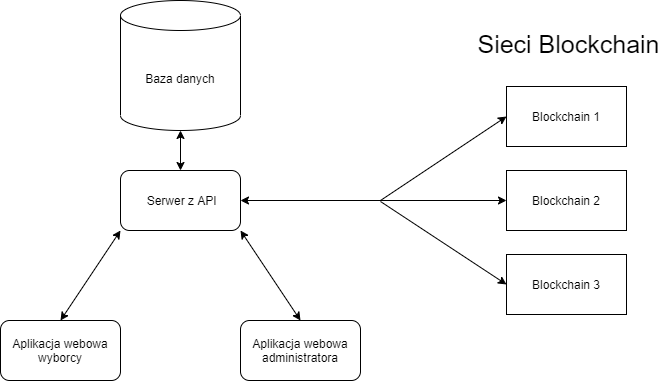
\includegraphics[width=\textwidth]{images/modules.png}
	\caption{Schemat przedstawiający komponenty systemu.}
\end {figure}

Taki podział systemu umożliwia wykorzystanie sieci Blockchain. Proces przeprowadzania wyborów jest zcentralizowany, a sieć Blockchain, która odpowiada za zapisanie wyników wyborów jest rozproszona.

\subsection{Architektura sieci Blockchain}

Sieć Blockchain to grupa serwerów, które wymieniają się informacjami. Komunikacja głównie odbywa się w celu przesłania zawartości nowego bloku, synchronizacji danych i dodania nowego węzła do sieci.

\section{Struktury danych}

W systemie można wyróżnić dwie struktury danych, które w znaczny sposób wpływają na zachowanie systemu. W tym podrozdziale omówiono implementację i zastoswania tych struktur danych.

\newpage

\subsection{Łańcuch bloków}

Za dostarczenie odpowiedniej struktury łańcucha bloków odpowiedzialne są klasy Block i ChainRepository. Listing 5.1 przedstawia klasę Block, która jest reprezentacją pojedynczego bloku. Każdy blok jest odpowiedzialny za przechowywanie głosu wyborczego. Głos jest przechowywany w polu data. Pole timestamp przechowuje datę utworzenia bloku w łańcuchu. W łańcuchu bloków, każdy blok posiada odniesienie do hasza poprzedniego bloku, w tej implementacji zajmuje się tym pole prevHash. Klasa Block posiada również pole nonce, którego zastosowanie zostało omówione w rozdziale dotyczącym algorytmów (5.3.1 Proof of Work).

\begin{lstlisting}[style=ES6, caption={Klasa Block.}]
class Block {
  index: number
  timestamp: string
  nonce: number
  prevHash: string
  data: string

  constructor (index: number,
 		timestamp: string,
 		nonce: number,
 		prevHash: string,
	 	data: string) {
    this.index = index
    this.timestamp = timestamp
    this.nonce = nonce
    this.prevHash = prevHash
    this.data = data
  }
}
\end{lstlisting}

Klasa ChainRepository (przedstawiona w listingu 5.2) odpowiada za przechowywanie łańcucha bloków i jego udostępnianie. Aby zapewnić spójność danych, ułatwienie dostępu i ograniczenie zużycia pamięci, w programie istnieje tylko jedna instancja tej klasy. W tym celu wykorzystano wzorzec projektowy Singleton. Z punktu widzenia łańcucha bloków istotne jest pole chain, które w tablicy przechowuje bloki. Klasa udostępnia metodę addBlock, która pozwala na dodawanie nowego bloku na początek tablicy, zgodnie z regułą tworzenia łańcucha bloków. Dodatkowo klasa posiada prywatną metodę \textit{createGenesisBlock}, która tworzy pierwszy blok łańcucha, którego zawartość nie przechowuje istotnych danych. Metoda wywoływana jest podczas tworzenia instancji ChainRepository.

\begin{lstlisting}[style=ES6, caption={Klasa ChainRepository.}]
class ChainRepository {
  public static instance: ChainRepository
  private chain: Block[]

  private constructor () {
    this.chain = new Array<Block>()
    this.createGenesisBlock()
  }

  public static getInstance (): ChainRepository {
    if (!ChainRepository.instance) {
      ChainRepository.instance = new ChainRepository()
    }
    return ChainRepository.instance
  }

  public addBlock (block: Block) {
    this.chain.push(block)
  }

  private createGenesisBlock () {
    const block 
	= new Block(this.chain.length, '0', 0, '0', 'genesis')

    this.chain.push(block)
  }
/* ... Getters and setters*/
}
\end{lstlisting}

Za zapewnienie poprawnego utworzenia nowego bloku odpowiedzialna jest metoda \textit{createNewBlock} (Listing 5.3), która należy do klasy Blockchain. Metoda przyjmuje następujące paramtry: \textit{nonce}, \textit{prevBlock} i \textit{data}. Z parametru \textit{prevBlock} wyliczany jest hash, za pomocą metody \textit{getHash}. Jest to hash poprzedniego bloku, który przypisywany jest do pola prevHash tworzonego bloku.

\begin{lstlisting}[style=ES6, caption={Fragment klasy Blockchain.}]
abstract class Blockchain {
  protected blockchain: ChainRepository

  public createNewBlock (nonce: number,  prevBlock: Block, 
					data: string): Block {
    const blockchain = this.blockchain.getChain()
    const chainLength = blockchain.length
    const prevHash = this.getHash(prevBlock)
    const date = Date.now().toString()

    const block = new Block(chainLength, date, nonce,
		 prevHash, data)

    return block
  }

  protected getHash (block: Block): string {
    const inputWord = block.toString()
    const hash = SHA256(inputWord).toString()
    return hash
  }
 /* ...  */
}
\end{lstlisting}

Tak skonstruowany blok jest gotowy do dodania do łańcucha. Dodawanie bloku jest realizowane za pomocą metody \textit{addBlock}, z klasy \textit{ChainRepository}.

\subsection{Baza danych}

W projekcie wykorzystano relacyjną bazę danych. Taka struktura danych pozwala na uporządkowanie danych w relacje pomiędzy tabelami. Rysunek 5.2 przedstawia schemat relacyjnego modelu wykorzystanej bazy danych.

\begin{figure}[h]
    	\centering
	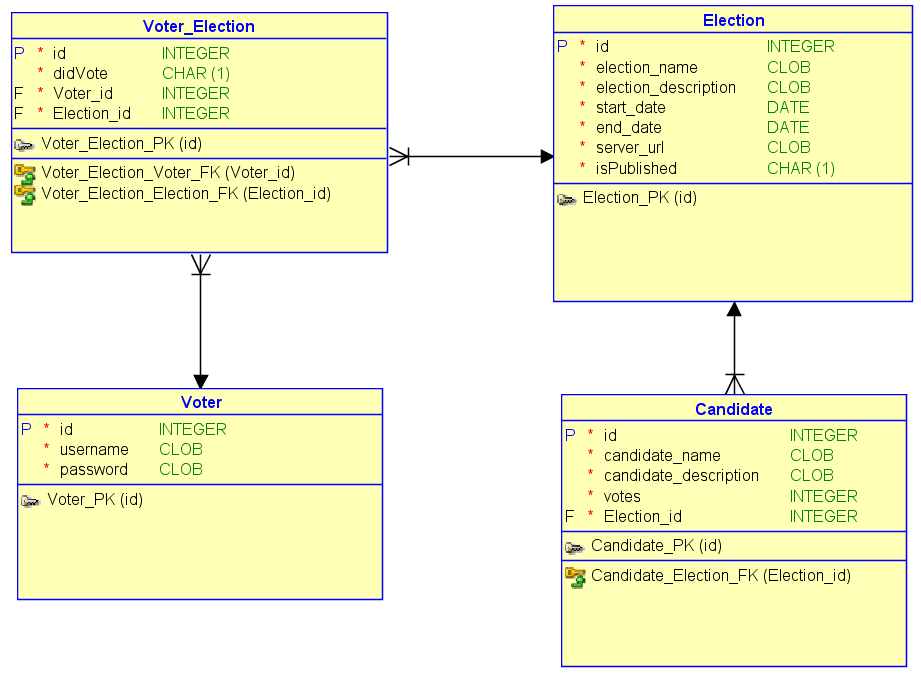
\includegraphics[width=\textwidth]{images/Relational.png}
	\caption{Schemat przedstawiający relacyjny schemat bazy danych.}
\end {figure}

Utworzona baza danych dzieli się na część odpowiadającą za przeprowadzenie wyborów oraz bank haseł i ról użytkowników. Tabele \textit{ADMIN} i \textit{VOTER} odpowiadają aktorom systemu. Na podstawie tych tabel można dokonać autoryzacji użytkownika systemu i przydzielić mu odpowiednią rolę, która zapewnia dostęp do zasobów. Dodatkowo tabela \textit{VOTER} jest połączona relacją wiele do wielu z tabelą \textit{ELECTION}. W wyniku realcji wiele do wielu powstała tabela łącznikowa \textit{VOTER\_ELECTION}, która pozwala podzielić relację wiele do wielu, na dwie relacje jeden do wielu. Tabela \textit{VOTER\_ELECTION} pozwala na przypisanie odpowiedniego wyborcy do odpowiednich wyborów. Dodatkowo tabela przechowuje informację o oddaniu głosu przez wyborcę, w polu \textit{DID\_VOTE}.

Pozostała część tabel odpowiada za przechowywanie danych dotyczących bezpośrednio wyborów. Zadaniem tabeli \textit{ELECTION} jest składowanie danych dotyczących konfiguracji wyborów. 
Konfiguracji mogą podlegać:
\begin{itemize}
	\item \textit{ELECTION\_NAME} - tytuł wyborów,
	\item \textit{ELECTION\_DESCRIPTION} - opis dotyczący wyborów,
	\item \textit{START\_DATE} - data rozpoczęcia wyborów,
	\item \textit{END\_DATE} - data zakończenia wyborów,
	\item \textit{SERVER\_URL} - adres zewnętrznego serwera sieci Blockchain, na który wysłane są głosy wyborców,
	\item kandydaci - zbiór kandydatów, którzy biorą udział w wyborach, jest reprezentowany jako relacja jeden do wielu z tabelą \textit{CANDIDATE}.
\end{itemize}

Dodatkowo w tabeli znajduje się również pole \textit{IS\_PUBLISHED} typu \textit{Boolean}, które odpowiada za oznaczenie stanu wyborów jako opublikowane lub nieopublikowane. System wykorzystuje tę informację do zakończenia wyborów i udostępnienia ich wyników.

Tabela \textit{CANDIDATE} reprezentuje kandydata, którego dane i opis definiują pola \textit{CANDIDATE\_NAME} i \textit{CANDIDATE\_DESCRIPTION}. Tabela posiada również pole \textit{VOTES}, które po zakończeniu wyborów uzupełniane jest o liczbę zdobytych głosów, przez danego kandydata.
\section{Algorytmy}

W podrozdziale algoytmy opisano implementacje algorytmów utrzymania konsensusu w sieci Blockchain. Każdy węzeł sieci Blockchain pozwala na wybranie algorytmu konsensusu, w którym będzie pracował.

\subsection{Proof of Work}



\subsection{Proof of Authority}
listingi kodu
\section{Zastosowane wzorce projektowe}
listingi kodu
\chapter{Testowanie}

\begin{thebibliography}{99}
\bibitem{pa} Ankit Patel:
\emph{English \TeX},
https://medium.com/@ankit\_233/history-of-the-blockchain-1991-38d6d4c3420c

\bibitem{bitcoin} Academy Binance: Czym jest Bitcoin?
\emph{Polski \TeX},
https://academy.binance.com/pl/articles/what-is-bitcoin\#what-is-bitcoin

\bibitem{business} Vadapalli, Ravindhar:
\emph{English \TeX},
BLOCKCHAIN FUNDAMENTALS TEXT BOOK Fundamentals of Blockchain s. 10

\bibitem{4-concepts} Vadapalli, Ravindhar:
\emph{English \TeX},
BLOCKCHAIN FUNDAMENTALS TEXT BOOK Fundamentals of Blockchain s. 19

\bibitem{bitcoin-vs-blockchain} Academy Binance: Jaka jest różnica między Blockchainem a Bitcoinem?
\emph{English \TeX},
https://academy.binance.com/pl/articles/difference-between-blockchain-and-bitcoin

\bibitem{hash} ZESZYTY NAUKOWE AKADEMII MARYNARKI WOJENNEJ
ROK LIV NR 2 (193) 2013  Przemysław Rodwald : KRYPTOGRAFICZNE FUNKCJE SKRÓTU
\emph{English \TeX},
 s. 92

\bibitem{pow-bitcoin} Andrew Tar: Proof-of-Work, Explained. 2018.
\emph{English \TeX},  https://cointelegraph.com/explained/proof-of-work-explained

\bibitem{elctricity-bitcoin} Bitcoin Mining. 2017. 
\emph{English \TeX}, https://powercompare.co.uk/bitcoin/

\bibitem{nodes} Academy Binance: Węzły (nodes) - czym są i jak działają?
\emph{Polski \TeX},https://academy.binance.com/pl/articles/what-are-nodes

\bibitem{CBECI} Cambridge Bitcoin Electricity Consumption Index
\emph{English \TeX},https://www.epe.admin.cam.ac.uk/cambridge-bitcoin-electricity-consumption-index-cbeci

\bibitem{atack51} Sarwar Sayeed and Hector Marco-Gisbert: Assessing Blockchain Consensus and Security Mechanisms against the 51\% Attack
\emph{English \TeX} https://www.mdpi.com/2076-3417/9/9/1788/htm

\bibitem{PKO} PKO BP wdraża nową wersję trwałego nośnika. To pierwsze takie rozwiązanie w Europie
\emph{Polski \TeX} https://fintek.pl/pko-bp-wdraza-nowa-wersje-trwalego-nosnika-to-pierwsze-takie-rozwiazanie-w-europie/

\bibitem{PKO-SMART}BLOCKCHAIN W PKO BANKU POLSKIM
\emph{Polski \TeX} https://fintech.pkobp.pl/blockchain-w-banku/

\bibitem{sp-han}https://www.lexlege.pl/ksh/oddzial-3-walne-zgromadzenie/57/
\emph{Polski \TeX} Kodeks Spółek Handlowych Art. 402. Tryb zwoływania walnego zgromadzenia

\bibitem{eVoting-dzialanie} https://www.kdpw.pl/pl/uslugi/Walne\_zgromadzenia/Strony/Jak-to-dziala.aspx
\emph{Polski \TeX} Walne zgromadzenia. eVoting - Jak to działa?

\bibitem{smart-contract} https://academy.binance.com/pl/articles/what-are-smart-contracts
\emph{Polski \TeX} Co to Smart Kontrakt?


\end{thebibliography}



\end{document}
